%%% -*- Mode: LaTeX; -*-
\chapter{Central Limit Theorem}
\label{ch:clt}

In this chapter, we show the formalisation of Lyapunov's form of Central Limit Theorem (CLT) in HOL4. We closely follow the textbook proof by Chung~\cite{Chung:2001}, employing primarily measure-theoretic techniques, Lindeberg's replacement principle, and Taylor expansions in explicit form. The general idea is to prove that the distribution of the normalised sum of independent random variables converges to a standard normal distribution under the Lyapunov condition.

The proof structure naturally divides into several steps, as shown in the figure below. First, we define the setup formally, e.g., probability spaces, independence, and moment conditions. Second, we introduce an auxiliary sequence of Gaussian random variables with the same variance structure as the original sequence but which are easier to manage in terms of distributional properties. The key strategy, referred to as the Lindeberg replacement trick, systematically replaces the original variables with the auxiliary variables and bounds the resulting error. Taylor's theorem gives us explicit error terms, while Lyapunov's inequality and Big-O estimates bound the third moment terms. Lastly, this sequence of approximations immediately gives us the desired convergence in distribution.

\begin{figure}[h!]
  \caption{Proof Structure}
  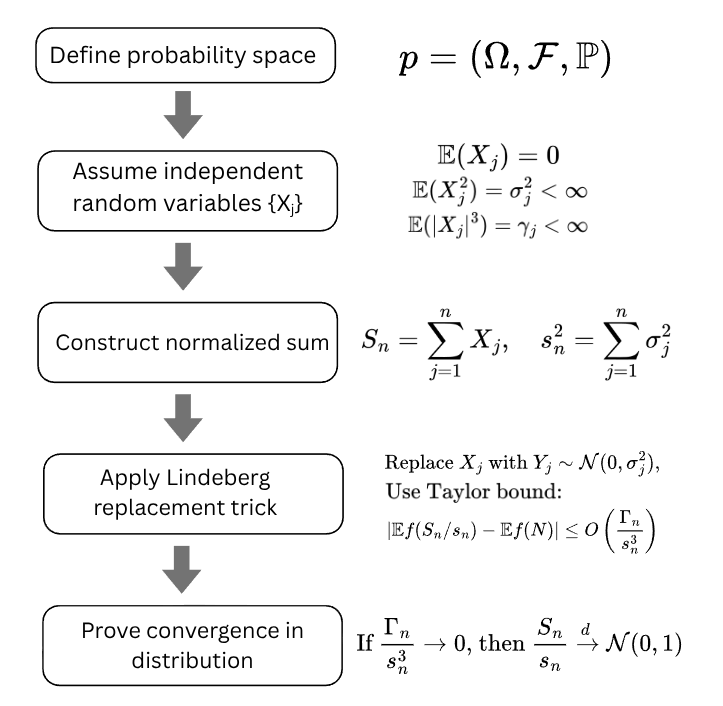
\includegraphics[width=7cm]{./img/method.png}
  \centering
\end{figure}

\section {Informal Proof}

To prove the Central Limit Theorem for a single sequence of independent (but not necessarily identically distributed) random variables $\{X_j\}_{1 \leq j \leq n}$, we apply the Lindeberg replacement method. Each $X_j$ is assumed to satisfy:

\[
\mathbb{E}[X_j] = 0, \quad \mathbb{E}[X_j^2] = \sigma_j^2 < \infty, \quad \mathbb{E}[|X_j|^3] = \gamma_j < \infty.
\]

Define the cumulative sums:

\[
S_n = \sum_{j=1}^n X_j, \quad s_n^2 = \sum_{j=1}^n \sigma_j^2, \quad \Gamma_n = \sum_{j=1}^n \gamma_j.
\]

We aim to prove that if:

\[
\frac{\Gamma_n}{s_n^3} \to 0,
\]

then the normalized sum $S_n / s_n$ converges in distribution to the standard normal.
Notationally, we write:

\[
\frac{S_n}{s_n} \xrightarrow{d} \mathcal{N}(0,1).
\]

\subsection{Replacement Strategy}

The idea is to approximate the sum $X_1 + \cdots + X_n$ by gradually replacing each $X_j$ with a corresponding independent normal variable $Y_j \sim \mathcal{N}(0, \sigma_j^2)$. Let all the $X_j$'s and $Y_j$'s be totally independent.

Define for each $j$:

\[
Z_j = Y_1 + \cdots + Y_{j-1} + X_j + \cdots + X_n,
\quad
Z_{j+1} = Y_1 + \cdots + Y_j + X_{j+1} + \cdots + X_n.
\]

So the difference $Z_j - Z_{j+1} = X_j - Y_j$ replaces one variable at a time.

Then:

\[
\mathbb{E}\left[ f\left(\frac{S_n}{s_n} \right) \right] - \mathbb{E}\left[ f\left(\frac{Y_1 + \cdots + Y_n}{s_n} \right) \right]
= \sum_{j=1}^n \left(
\mathbb{E}\left[f\left( \frac{X_j + Z_j}{s_n} \right)\right]
- \mathbb{E}\left[f\left( \frac{Y_j + Z_j}{s_n} \right)\right]
\right)
\]

\subsection{Taylor Expansion Bound}

Using Taylor's theorem and the fact that $f \in C^3_b$ (bounded continuous functions with bounded derivatives up to order 3), we bound the difference:

\[
\left| \mathbb{E}\left[f\left( \frac{X_j + Z_j}{s_n} \right)\right] -
       \mathbb{E}\left[f\left( \frac{Y_j + Z_j}{s_n} \right)\right]
\right| \leq
\frac{M}{6 s_n^3} \left( \mathbb{E}[|X_j|^3] + \mathbb{E}[|Y_j|^3] \right),
\]

for  $M = \sup_{x \in \mathbb{R}} \left| f^{(3)}(x) \right|$.

This constant $M$ reflects the maximum curvature of $f$, and controls the Taylor remainder in the third-order expansion.

Summing over $j$, we get:

\[
\left| \mathbb{E}\left[f\left( \frac{S_n}{s_n} \right) \right] -
       \mathbb{E}[f(N)]
\right| \leq
\frac{M}{6 s_n^3} \sum_{j=1}^n \left( \gamma_j + c \sigma_j^3 \right),
\]

where $N \sim \mathcal{N}(0, 1)$ and $c$ is a constant depending on the third moment of standard normal.

By Lyapunov’s inequality, $\sigma_j^3 \leq \gamma_j$, so the right-hand side is $O(\Gamma_n / s_n^3)$, which tends to zero. This proves $S_n / s_n \xrightarrow{d} N(0,1)$.


\section {Construction of Auxiliary Sequence}

To carry out the Lindeberg replacement method, we need to introduce an auxiliary sequence $\{Y_j\}$ of Gaussian random variables that are independent and have the same variance structure as the original $\{X_j\}$. The goal is to build these $Y_j$ over a new probability space that allows us to reason about both $X_j$ and $Y_j$ simultaneously.

\begin{theorem}[Existence of independent variables]
\label{thm:existence-of-indep-vars}
Let $D$ be a function that gives positive variances for $n > 0$ dimensions — that is, for each index $i < n$, $D(i) > 0$.

Then, there exists a new probability space $p'$, and a sequence of random variables $Y_0, Y_1, \dots, Y_{n-1}$ defined on that space such that:
\begin{itemize}
\item Each $Y_i$ is a normal random variable with mean 0 and variance $D(i)$
\item The random variables $Y_0, \dots, Y_{n-1}$ are independent from each other
\end{itemize}
\end{theorem}

Or formally,

\begin{hol}
  \begin{alltt}
    Theorem existence\_of\_indep\_vars :
    \(\!\!\!{\turn}\!\!\!\!\) \(\forall\)(p :\(\alpha\) m\_space) N (D :num \(\rightarrow\) real) n.
    prob\_space p \(\land\) 0 < n \(\land\) ext\_normal\_rv N p 0 1 \(\land\)
    (\(\forall\)i. i < n \(\Rightarrow\) 0 < (D i)) \(\Rightarrow\)
    \(\exists\)(p' :\(\alpha\) list m\_space) Y.
    prob\_space p' \(\land\)
    (\(\forall\)(i :num). i < n \(\Rightarrow\) ext\_normal\_rv (Y i) p' 0 (D i)) \(\land\)
    indep\_vars p' Y (\(\lambda\)i. Borel) (count n)
  \end{alltt}
\end{hol}

The classic idea, as presented in Fremlin’s Measure Theory~\cite{fremlinmeasure}, is to construct the product space $\Omega' = \Omega \times \mathbb{R}^n$, where $\Omega$ is the original probability space carrying the variables $X_1, \dots, X_n$, and $\mathbb{R}^n$ is equipped with a standard Gaussian product measure. Each component of this product then hosts one of the auxiliary Gaussian variables. This idea guarantees that we can preserve the distribution of $X_j$ while augmenting the space with new independent $Y_j \sim \mathcal{N}(0, \sigma_j^2)$.

In our formalisation, we adapt this idea to HOL4 by explicitly constructing two independent probability spaces:
\begin{itemize}
    \item $p_1$, hosting the original sequence $\{X_i\}_{i < n}$,
    \item $p_2$, hosting the auxiliary sequence $\{Y_i\}_{i < n}$, assumed to be independent and Gaussian.
\end{itemize}

We then take their product measure $p = p_1 \times p_2$, which remains a valid probability space thanks to the existing \holtxt{existence\_of\_prod\_prob\_space} theorem.

\begin{hol}
  \begin{alltt}
    Theorem existence\_of\_prod\_prob\_space :
    \(\!\!\!{\turn}\!\!\!\!\) \(\forall\)p1 p2.
    prob\_space p1 \(\land\) prob\_space p2 \(\Rightarrow\)
    \(\exists\)p. p = p1 \(\times\) p2 \(\land\) prob\_space p \(\land\)
    (\(\forall\)e1 e2.
    e1 \(\in\) events p1 \(\land\) e2 \(\in\) events p2 \(\Rightarrow\)
    e1 \(\times\) e2 \(\in\) events p \(\land\)
    prob p (e1 \(\times\) e2) = prob p1 e1 * prob p2 e2)
  \end{alltt}
\end{hol}

Within this product space, we define:
\begin{itemize}
    \item $X'_i = X_i \circ \texttt{FST}$, and
    \item $Y'_i = Y_i \circ \texttt{SND}$,
\end{itemize}

as random variables on $p$, so that their marginal behaviours match the originals. Finally, we interleave these into a single indexed family:

\[
    Z_i(x) =
    \begin{cases}
      X'_i(x), & \text{if } i < n \\
      Y'_{i-n}(x), & \text{if } n \leq i < 2n
    \end{cases}
\]

We formally prove that the sequence $\{Z_i\}_{i < 2n}$ is a family of independent real-valued random variables over the product probability space $p$. This construction ensures that:

\begin{itemize}
\item The first $n$ components $\{Z_i\}_{i < n}$ correspond exactly to $X_i$,
\item The remaining $\{Z_i\}_{n \leq i < 2n}$ are the auxiliary $Y_j$, with identical variance structure,
\item All variables are mutually independent.
\end{itemize}

This leads to the following formal result in HOL4, which guarantees the existence of such a product probability space and the sequence $Z_i$ combining both original and auxiliary components.

\begin{theorem}[Construction of auxiliary sequence]
  \label{thm:construct-aux-seq}
  There exists a product probability space $p = p_1 \times p_2$ supporting two independent sequences of random variables $X'_i = X_i \circ \texttt{FST}$ and $Y'_i = Y_i \circ \texttt{SND}$ such that the interleaved sequence $Z_i$ combines both and preserves mutual independence and variance structure.
\end{theorem}

Or, formally:

\begin{hol}
  \begin{alltt}
    Theorem construct\_auxiliary\_seq :
    \(\!\!\!{\turn}\!\!\!\!\) \(\forall\)p1 (p2 :'a list m\_space) X Y (n \:num).
    prob\_space p1 \(\land\) prob\_space p2 \(\land\) 0 < n \(\land\)
    (\(\forall\)i. i < n \(\Rightarrow\) real\_random\_variable (X i) p1) \(\land\)
    (\(\forall\)i. i < n \(\Rightarrow\) real\_random\_variable (Y i) p2) \(\land\)
    indep\_vars p1 X (\(\lambda\)i. Borel) (count n) \(\land\)
    indep\_vars p2 Y (\(\lambda\)i. Borel) (count n) \(\Rightarrow\)
    \(\exists\)p X' Y' Z.
    (p = p1 CROSS p2) \(\land\)
    (X' = \(\lambda\)i. X i \(\circ\) FST) \(\land\)
    (Y' = \(\lambda\)i. Y i \(\circ\) SND) \(\land\)
    prob\_space p \(\land\)
    (\(\forall\)i. i < n \(\Rightarrow\) real\_random\_variable (X' i) p) \(\land\)
    (\(\forall\)i. i < n \(\Rightarrow\) real\_random\_variable (Y' i) p) \(\land\)
    (Z = \(\lambda\)i x. if i < n then X' i x else Y' (i - n) x) \(\land\)
    indep\_vars p Z (\(\lambda\)(i \:num). Borel) (count (2 \* n))
  \end{alltt}
\end{hol}

\section {Taylor Expansion Bounds}

After constructing the auxiliary sequence $\{Y_j\}$ of independent normal variables matching the variances of $\{X_j\}$, the next step is to control the difference in expectations:

\[
\mathbb{E}[f(S_n / s_n)] - \mathbb{E}[f(G_n / s_n)],
\]

where $S_n = \sum_{j=0}^{n-1} X_j$, and $G_n = \sum_{j=0}^{n-1} Y_j$. We do this by replacing one term at a time, writing the difference as a telescoping sum:

\[
\sum_{j=0}^{n-1} \left(
\mathbb{E}\left[f\left(\frac{X_j + Z_j}{s_n}\right)\right]
-
\mathbb{E}\left[f\left(\frac{Y_j + Z_j}{s_n}\right)\right]
\right),
\]

where $Z_j$ is the partial sum involving all terms except $X_j$ or $Y_j$.
To estimate each difference, we use Taylor's theorem with remainder.


\subsection{Taylor Expansion Theorems}

To formally bound the error, we need two main ingredients:

\begin{theorem}[Taylor’s Theorem]
  \label{thm:taylor}
Let $f : \mathbb{R} \to \mathbb{R}$ be $n$-times differentiable on an interval $[a, x]$. Then there exists some $t \in (a, x)$ such that:

\[
f(x) =
\sum_{m=0}^{n-1} \frac{f^{(m)}(a)}{m!} (x - a)^m +
\frac{f^{(n)}(t)}{n!} (x - a)^n.
\]

In our setting, we focus on the case $n = 3$, so:

\[
f(a + h) =
f(a) + f'(a)h + \frac{1}{2}f''(a)h^2 + \frac{1}{6}f^{(3)}(t)h^3.
\]
\end{theorem}

This is captured in HOL4 as:

\begin{hol}
  \begin{alltt}
    Theorem TAYLOR\_THEOREM :
    \(\!\!\!{\turn}\!\!\!\!\) \(\forall\)f a x n.
    a < x \(\land\) 0 < n \(\land\)
    (\(\forall\)m t. m < n \(\land\) a \(\le\) t \(\land\) t \(\le\) x \(\Rightarrow\)
    higher\_differentiable (SUC m) f t) \(\Rightarrow\)
    \(\exists\)t. a < t \(\land\) t < x \(\land\)
    f x =
    sum (0,n) (\(\lambda\)m. diff m f a / \&FACT m * (x \({-}\) a) pow m) +
    diff n f t / \&FACT n * (x \({-}\) a) pow n
  \end{alltt}
\end{hol}

\begin{theorem}[Taylor Remainder Bound]
\label{thm:taylor-remainder}
The Taylor remainder theorem describes the difference between a function and its Taylor polynomial. Suppose $f : \mathbb{R} \to \mathbb{R}$ is $n$-times differentiable on an interval containing $a$ and $x = a + h$. The function value $f(x)$ can be written as:

\[
f(x) = \sum_{m=0}^{n-1} \frac{f^{(m)}(a)}{m!} h^m + R_n(h),
\]

where $R_n(h)$ is the remainder term. Taylor's theorem guarantees that there exists some $t$ between $a$ and $x$ such that:

\[
R_n(h) = \frac{f^{(n)}(t)}{n!} h^n.
\]
\end{theorem}

Or, formally:
\begin{hol}
  \begin{alltt}
    Theorem TAYLOR\_REMAINDER :
    \(\!\!\!{\turn}\!\!\!\!\) \(\forall\)n x f. \(\exists\)M t.
    abs (Normal (diff n f t)) \(\le\) M \(\Rightarrow\)
    abs (Normal (diff n f t / \&FACT n) * Normal x pow n) \(\le\)
    M / Normal (\&FACT n) * abs (Normal x) pow n
  \end{alltt}
\end{hol}

Assume $f \in C^3_b$, that is, $f$ has bounded third derivative over $\mathbb{R}$, and let:

\[
M = \sup_{x \in \mathbb{R}} |f^{(3)}(x)|.
\]

Then the remainder term satisfies:

\[
\left| f(a + h) - f(a) - f'(a)h - \frac{1}{2}f''(a)h^2 \right|
\leq \frac{M}{6} |h|^3.
\]

This is formalised as:
\begin{hol}
  \begin{alltt}
    Theorem TAYLOR\_THIRD\_ORDER\_BOUND :
    \(\!\!\!{\turn}\!\!\!\!\) \(\forall\)f a h M.
    f \(\in\) CnR 3 \(\land\)
    M = sup (IMAGE (\(\lambda\)t. abs (Normal (diff 3 f t))) \(\mathbb{U}\)(:\(\real\))) \(\Rightarrow\)
    abs (Normal (f (a + h) \({-}\) f a \({-}\) diff 1 f a * h \({-}\) 1 / 2 * diff 2 f a * h pow 2)) \(\le\)
    M / 6 * abs (Normal h) pow 3
  \end{alltt}
\end{hol}

This bound will be applied to the difference $f(X_j + Z_j) - f(Y_j + Z_j)$, treating $X_j - Y_j$ as a small perturbation.

\section{Formal Lindeberg Replacement Lemma}

After constructing the auxiliary sequence $\{Y_j\}$ and bounding the Taylor expansion error for each replacement, we now formalise the full Lindeberg replacement argument. This step accumulates the errors introduced when replacing each original variable $X_j$ by the corresponding auxiliary normal variable $Y_j$, and shows that the total error vanishes under Lyapunov's condition.

\subsection{Error Decomposition via Telescoping Sum}

Let $S_n = \sum_{j=0}^{n-1} X_j$ and $G_n = \sum_{j=0}^{n-1} Y_j$, and fix a function $f : \mathbb{R} \to \mathbb{R}$ in the class $C^3_b$, i.e., $f$ is three times differentiable with all derivatives bounded. Our goal is to estimate the difference:

\[
\left| \mathbb{E}\left[f\left(\frac{S_n}{s_n}\right)\right]
     - \mathbb{E}\left[f\left(\frac{G_n}{s_n}\right)\right] \right|.
\]

Following the informal argument, we express this difference as a telescoping sum:

\[
\sum_{j=0}^{n-1} \left(
\mathbb{E}\left[f\left(\frac{X_j + Z_j}{s_n}\right)\right]
-
\mathbb{E}\left[f\left(\frac{Y_j + Z_j}{s_n}\right)\right]
\right),
\]

where each $Z_j$ represents the sum of the remaining variables (excluding $X_j$ and $Y_j$), and is assumed independent from both.

Each term in this sum is then bounded using Taylor's theorem as shown in the previous section.

\begin{lemma}[Measurability of Partial Sums]
  Given real-valued integrable random variables $ X_0, \dots, X_{n-1} $ and $ Y_0, \dots, Y_{n-1} $, define:
  \[
  Z_j(x) = \sum_{i<j} Y_i(x) + \sum_{j \le i < n} X_i(x).
  \]
  Then each $ Z_j $ is also a real random variable and integrable.
\end{lemma}


This lemma ensures that each such function $Z_j$ remains a real random variable and integrable:

\begin{hol}
\begin{alltt}
Theorem clt\_partial\_sum\_lemma :
\(\!\!\!{\turn}\!\!\!\!\) \(\forall\)p X Y Z f n.
prob\_space p \(\land\)
(\(\forall\)i. i < n \(\Rightarrow\)
  real\_random\_variable (X i) p \(\land\)
  real\_random\_variable (Y i) p \(\land\)
  integrable p (X i) \(\land\)
  integrable p (Y i)) \(\Rightarrow\)
(\(\forall\)j. j < n \(\Rightarrow\)
  \(\forall\)Z. Z =
    (\(\lambda\)j x.
      if x \(\in\) p\_space p then
        \(\sum\) (\(\lambda\)i. Y i x) (count j) +
        \(\sum\) (\(\lambda\)i. X i x) (count n \(\setminus\) count j)
      else 0) \(\Rightarrow\)
    real\_random\_variable (Z j) p \(\land\) integrable p (Z j))
\end{alltt}
\end{hol}

This result guarantees that the hybrid sum $Z_j$, required for the Lindeberg replacement trick, is well-defined and suitable for expectation bounds.

\begin{lemma}[Telescoping Sum Identity]
  For any real-valued function \( f \) where each term is finite, we have:
  \[
  \sum_{j = 0}^{n-1} (f(j) - f(j+1)) = f(0) - f(n).
  \]
\end{lemma}

This is formalised in HOL4 as:

\begin{hol}
\begin{alltt}
Theorem SUM\_SUB\_GEN :
\(\!\!\!{\turn}\!\!\!\!\) \(\forall\)f n.
(\(\forall\)x. f x \(\ne\) -\(\infty\) \(\land\) f x \(\ne\) +\(\infty\)) \(\Rightarrow\)
\(\sum\) (\(\lambda\)j. f j \({-}\) f (j + 1)) (count n) = f 0 \({-}\) f n
\end{alltt}
\end{hol}

This identity is especially useful in simplifying the error terms expressed as a telescoping sum when estimating differences between expectations.

\begin{theorem}[Lindeberg Replacement Lemma]
  \label{thm:lindeberg-replacement}
  Let $X_j$, $Y_j$ be independent sequences of real random variables with bounded third moments, and let $f \in C^3_b$. Then the total replacement error between $X_j$ and $Y_j$ when replacing them one by one is bounded as follows...
\end{theorem}

In HOL4, it states as:

\begin{hol}
\begin{alltt}
Theorem clt\_Lindeberg\_replacement\_trick\_bounded[local] :
\(\!\!\!{\turn}\!\!\!\!\) \(\forall\)p X Y f s n.
prob\_space p \(\land\)
f \(\in\) CnR 3 \(\land\)
(\(\forall\)i. i < n \(\Rightarrow\)
  real\_random\_variable (X i) p \(\land\)
  real\_random\_variable (Y i) p \(\land\)
  integrable p (X i) \(\land\)
  integrable p (Y i)) \(\land\)
0 < s n \(\land\) s n \(\ne\) +\(\infty\) \(\land\) s n \(\ne\) -\(\infty\) \(\land\)
(\(\forall\)j. j < n \(\Rightarrow\)
  (\(\forall\)Z. Z = (\(\lambda\)j x. if x \(\in\) p\_space p then
                      \(\sum\) (\(\lambda\)i. Y i x) (count j) +
                      \(\sum\) (\(\lambda\)i. X i x) (count n DIFF count1 j)
                   else 0) \(\Rightarrow\)
    expectation p (Normal \(\circ\) f \(\circ\) real \(\circ\)
                   (\(\lambda\)x. \(\sum\) (\(\lambda\)i. X i x) (count n) / s n)) \({-}\)
    expectation p (Normal \(\circ\) f \(\circ\) real \(\circ\)
                   (\(\lambda\)x. \(\sum\) (\(\lambda\)i. Y i x) (count n) / s n)) =

    \(\sum\) (\(\lambda\)j.
      expectation p (Normal \(\circ\) f \(\circ\) real \(\circ\)
                     (\(\lambda\)x. (X j x + Z j x) / s n)) \({-}\)
      expectation p (Normal \(\circ\) f \(\circ\) real \(\circ\)
                     (\(\lambda\)x. (Y j x + Z j x) / s n))) (count n)))
\end{alltt}
\end{hol}

This theorem quantifies how the accumulated replacement error scales with the third moments of $X_j$ and $Y_j$, and the normalization constant $s_n$. The assumptions guarantee:

\begin{itemize}
\item \textbf{Independence}: Each pair $(X_j, Z_j)$ and $(Y_j, Z_j)$ are independent, which is crucial for separating expectations during Taylor expansion.
\item \textbf{Matching Second Moments}: Implicitly required for the expectation of quadratic terms to cancel out.
\item \textbf{Bounded Third Derivative}: Controlled via the supremum constant $M$ defined from the third derivative of $f$.
\end{itemize}

This theorem precisely formalises Equation (15) in the informal Chung proof. The right-hand side provides an upper bound on the total error in terms of third moments. Once we show that this upper bound tends to zero (which we do using Lyapunov’s condition in the next section), we conclude that the distribution of $S_n / s_n$ is close to that of $G_n / s_n$, which converges to standard normal.

Thus, this lemma acts as the bridge between the approximation via normal variables and the original non-Gaussian sequence.

\begin{figure}[h]
  \caption{Illustration of the Lindeberg replacement method}
  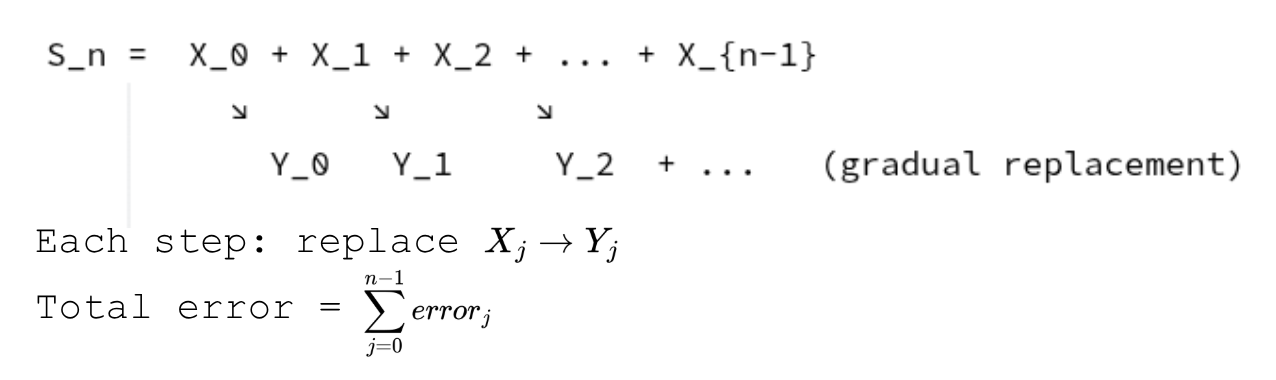
\includegraphics[width=12cm]{./img/replacement.png}
  \centering
\end{figure}


\section{Global Taylor Error Bound}

After expressing the Lindeberg replacement as a telescoping sum and bounding each replacement using Taylor’s theorem, we now combine those bounds into a single inequality. This step precisely captures the cumulative approximation error when replacing each $X_j$ by $Y_j$.

\subsection{Formal Statement of the Error Bound}

We define $f \in C^3_b$ as a test function with bounded third derivative. Let $X_j$, $Y_j$, and $Z_j$ be sequences of real random variables such that for each $j < n$:
\begin{itemize}
    \item $Z_j$ is independent of both $X_j$ and $Y_j$,
    \item $X_j$ and $Y_j$ are centered, share the same variance,
    \item third moments $\mathbb{E}[|X_j|^3]$ and $\mathbb{E}[|Y_j|^3]$ are finite.
\end{itemize}


Then the total error is bounded by:

\[
\left| \sum_{j=0}^{n-1}
\mathbb{E}\left[f\left(\frac{X_j + Z_j}{s_n} \right)\right] -
\mathbb{E}\left[f\left(\frac{Y_j + Z_j}{s_n} \right)\right]
\right| \leq \frac{M}{6 s_n^3}
\sum_{j=0}^{n-1} \left( \mathbb{E}[|X_j|^3] + \mathbb{E}[|Y_j|^3] \right)
\]

where $M = \sup_{x \in \mathbb{R}} |f^{(3)}(x)|$, and $s_n^2 = \sum_{j=0}^{n-1} \mathrm{Var}(X_j)$.

\begin{theorem}[Global Taylor Error Bound]
  \label{thm:taylor-error-bound}
  Given independent sequences $X_j$, $Y_j$, $Z_j$ with bounded third moments and a test function $f \in C^3_b$, the cumulative difference in expectations is bounded by the total third moments scaled by $s_n^{-3}$.
\end{theorem}

This is formalised in HOL4 as:

\begin{hol}
\begin{alltt}
Theorem clt\_lindeberg\_taylor\_error\_bound :
\(\!\!\!{\turn}\!\!\!\!\) \(\forall\)r X Y Z f M s n.
prob\_space r \(\land\)
(\(\forall\)(j :num). j < n \(\Rightarrow\)
  real\_random\_variable (X j) r \(\land\)
  real\_random\_variable (Y j) r \(\land\)
  real\_random\_variable (Z j) r \(\land\)
  integrable r (\(\lambda\)x. X j x) \(\land\)
  integrable r (\(\lambda\)x. Y j x) \(\land\)
  integrable r (\(\lambda\)x. Z j x) \(\land\)
  integrable r (\(\lambda\)x. (abs (X j x)) pow 3) \(\land\)
  integrable r (\(\lambda\)x. (abs (Y j x)) pow 3) \(\land\)
  indep\_vars r (X j) (Z j) Borel Borel \(\land\)
  indep\_vars r (Y j) (Z j) Borel Borel) \(\land\)
f \(\in\) CnR 3 \(\land\)
M = sup (IMAGE (\(\lambda\)t. abs (Normal (diff 3 f t))) UNIV) \(\land\)
0 < s n \(\land\) s n \(\ne\) +\(\infty\) \(\land\) s n \(\ne\) -\(\infty\) \(\Rightarrow\)
abs (\(\sum\) (\(\lambda\)j.
  expectation r (Normal \(\circ\) f \(\circ\) real \(\circ\) (\(\lambda\)x. (X j x + Z j x) / s n)) \({-}\)
  expectation r (Normal \(\circ\) f \(\circ\) real \(\circ\) (\(\lambda\)x. (Y j x + Z j x) / s n))) (count n)) \(\le\)
M / (6 * (s n) pow 3) *
\(\sum\) (\(\lambda\)j.
  expectation r (\(\lambda\)x. (abs (X j x)) pow 3 + (abs (Y j x)) pow 3)) (count n)
\end{alltt}
\end{hol}

This theorem completes the Lindeberg replacement method by quantifying the total replacement error via third moment control. As the Lyapunov condition ensures the RHS tends to zero, it follows that the difference in distributions of the original and auxiliary sums vanishes.

This theorem serves as the final analytic step before applying convergence theorems to conclude:

\[
\frac{S_n}{s_n} \xrightarrow{d} \mathcal{N}(0,1).
\]


\section{Lyapunov Condition and Third Moment Bound}

This section connects the Lyapunov condition with third moment estimates used in bounding the global Taylor approximation error. This connection ensures that the total error in the Lindeberg method vanishes asymptotically.

\begin{theorem}[Lyapunov Inequality]
  \label{thm:lyapunov-ineq}
  For a random variable $X$ with finite $r$-th and $r'$-th absolute moments where $0 < r < r'$, we have:
  \[
  \left( \mathbb{E}[|X|^r] \right)^{1/r} \le \left( \mathbb{E}[|X|^{r'}] \right)^{1/r'}.
  \]
\end{theorem}

In short, the $L^r$ norm of $X$ is bounded by its $L^{r'}$ norm. This allows us to control lower-order moments using higher-order ones — a key idea in proving convergence in distribution under Lyapunov conditions.


\subsection{Lyapunov Inequality for Integrals}

We begin with a basic inequality that bounds the $L^1$ norm of a function by its $L^p$ seminorm, scaled by the measure of the entire space. This is useful when estimating the first moment of a random variable in $L^p$ for $p > 1$.

\begin{hol}
\begin{alltt}
Theorem liapounov\_ineq\_lemma :
\(\!\!\!{\turn}\!\!\!\!\) \(\forall\)m u p.
measure\_space m \(\land\) measure m (m\_space m) < +\(\infty\) \(\land\)
1 < p \(\land\) p < +\(\infty\) \(\land\)
u \(\in\) lp\_space p m \(\Rightarrow\)
\(\int^+\) m (\(\lambda\)x. abs (u x)) \(\le\)
seminorm p m u * measure m (m\_space m) powr (1 \({-}\) inv p)
\end{alltt}
\end{hol}

\subsection{Comparing $L^p$ and $L^{p'}$ Seminorms}

The next two theorems compare $L^p$ seminorms when $p < p'$, assuming the measure space is finite.

\begin{hol}
\begin{alltt}
Theorem liapounov\_ineq :
\(\!\!\!{\turn}\!\!\!\!\) \(\forall\)m u r r'.
measure\_space m \(\land\)
u \(\in\) lp\_space r m \(\land\) u \(\in\) lp\_space r' m \(\land\)
measure m (m\_space m) < +\(\infty\) \(\land\)
0 < r \(\land\) r < r' \(\land\) r' < +\(\infty\) \(\Rightarrow\)
seminorm r m u \(\le\)
seminorm r' m u * measure m (m\_space m) powr (inv r \({-}\) inv r')
\end{alltt}
\end{hol}

In a probability space, where the total measure is 1, the inequality simplifies:

\begin{hol}
\begin{alltt}
Theorem liapounov\_ineq\_rv :
\(\!\!\!{\turn}\!\!\!\!\) \(\forall\)p u r r'.
prob\_space p \(\land\)
u \(\in\) lp\_space r p \(\land\) u \(\in\) lp\_space r' p \(\land\)
0 < r \(\land\) r < r' \(\land\) r' < +\(\infty\) \(\Rightarrow\)
seminorm r p u \(\le\) seminorm r' p u
\end{alltt}
\end{hol}

These inequalities help relate different moment conditions and are crucial when applying Lyapunov’s condition for the CLT.

\subsection{Variance Controlled by Third Moment}

We now state a bound showing that the third absolute moment dominates the cube of the standard deviation.

\begin{hol}
\begin{alltt}
Theorem clt\_liapounov\_upper\_bound :
\(\!\!\!{\turn}\!\!\!\!\) \(\forall\)p X Y.
prob\_space p \(\land\)
real\_random\_variable X p \(\land\)
expectation p (\(\lambda\)x. (abs (X x)) pow 3) < +\(\infty\) \(\Rightarrow\)
Normal (sqrt (real (variance p X))) pow 3 \(\le\)
expectation p (\(\lambda\)x. (abs (X x)) pow 3)
\end{alltt}
\end{hol}

In the CLT, we normalize the sum by $s_n^3 = \left( \sum_j \mathrm{Var}(X_j) \right)^{3/2}$. This bound ensures the denominator does not vanish too quickly, keeping the Taylor error under control.

\subsection{Exact Third Moment of a Gaussian Variable}

For the auxiliary sequence $Y_j \sim \mathcal{N}(0, \sigma^2)$, the third absolute moment is:

\[
\mathbb{E}[|X|^3] = \sqrt{\frac{8}{\pi}} \cdot \sigma^3,
\quad \text{for } X \sim \mathcal{N}(0, \sigma^2).
\]

Formally,
\begin{hol}
  \begin{alltt}
    Theorem ext\_normal\_rv\_abs\_third\_moment :
    \(\!\!\!{\turn}\!\!\!\!\) \(\forall\)p X sig. prob\_space p \(\land\) 0 < sig \(\land\)
    ext\_normal\_rv X p 0 sig \(\Rightarrow\)
    expectation p (\(\lambda\)x. abs (X x) pow 3) = sqrt (8 / Normal pi) * Normal (sig pow 3)
  \end{alltt}
\end{hol}

\noindent
\emph{Remark on Formalisation.}
This result relies on integration over unbounded domains and special functions such as the gamma function $\Gamma(z)$. While it is analytically correct and standard in probability theory, its full formalisation in HOL4 is not yet feasible. HOL4 is based entirely on the Lebesgue integral and currently lacks:

\begin{itemize}
    \item integration over $\mathbb{R}$ with non-trivial densities like the Gaussian,
    \item improper integrals as limits over infinite intervals,
    \item and complex-analytic foundations needed for $\Gamma(z)$ where $z \in \mathbb{C}$.
\end{itemize}

Although the Riemann and Lebesgue integrals often agree for well-behaved functions like $x \mapsto |x|^3 e^{-x^2/2}$, this equivalence is not formalised in HOL4. Therefore, we treat the equation

\[
\mathbb{E}[|X|^3] = \sqrt{\frac{8}{\pi}} \cdot \sigma^3
\]

as an \emph{informally justified assumption}, grounded in classical analysis. A full mechanisation is deferred to future work on HOL4’s measure and complex analysis libraries.

\subsubsection*{Informal Proof}

For $Z \sim \mathcal{N}(0, 1)$:

\[
\mathbb{E}[|Z|^3] = \frac{1}{\sqrt{2\pi}} \int_{-\infty}^\infty |x|^3 e^{-x^2/2} dx
= \frac{2}{\sqrt{2\pi}} \int_0^\infty x^3 e^{-x^2/2} dx.
\]

Change of variable $u = x^2/2$ gives:

\[
\int_0^\infty x^3 e^{-x^2/2} dx
= \int_0^\infty \sqrt{2u} \cdot 2u \cdot e^{-u} \cdot \frac{1}{\sqrt{2u}} du
= 2 \int_0^\infty u e^{-u} du = 2 \cdot \Gamma(2) = 2.
\]

So:

\[
\mathbb{E}[|Z|^3] = \frac{2}{\sqrt{2\pi}} \cdot 2 = \sqrt{\frac{8}{\pi}}.
\]

More generally, for any $\nu > -1$:

\[
\mathbb{E}[|Z|^\nu] = 2^{\nu/2} \cdot \frac{\Gamma\left( \frac{\nu + 1}{2} \right)}{\sqrt{\pi}}.
\]

See Winkelbauer \cite{winkelbauer2012moments} for a comprehensive derivation using special functions like Kummer's $\Phi$ and the parabolic cylinder function $D_\nu$.

\emph{Remarks on the Standard Normal Density}

The standard Gaussian density is:

\[
x \mapsto \frac{1}{\sqrt{2\pi}} e^{-x^2 / 2},
\]

which integrates to 1:

\[
\frac{1}{\sqrt{2\pi}} \int_{-\infty}^{+\infty} e^{-x^2 / 2} dx = 1.
\]

This confirms it defines a valid probability distribution. However, this fundamental fact is also not fully formalised in HOL4, due to limitations in its support for improper integrals over $\mathbb{R}$. We include it as an assumed classical result.

\subsection{Lyapunov Ratio in the CLT}

We now combine the third moment estimates into the Lyapunov ratio, which controls the Taylor approximation error in the CLT:

\[
\frac{\Gamma_n}{s_n^3}
= \frac{\sum_j \mathbb{E}[|X_j|^3]}{\left( \sum_j \mathrm{Var}(X_j) \right)^{3/2}}.
\]

Under the Lyapunov condition:

\[
\lim_{n \to \infty} \frac{\Gamma_n}{s_n^3} = 0,
\]

which ensures convergence in distribution to the standard normal law.

\subsection{Asymptotic Error Bound and Big-O Formalisation}

The total Taylor approximation error in the Lindeberg replacement scheme is bounded by the expression:

\begin{equation}
\label{eq:taylor-bound}
\frac{M}{6} \sum_{j = 1}^{n} \left( \frac{y_j}{s_n^3} + \frac{c \sigma_j^3}{s_n^3} \right),
\end{equation}

where \( y_j = \mathbb{E}[|X_j|^3] \), \( \sigma_j^2 = \text{Var}(X_j) \), and \( c = \sqrt{8/\pi} \) is the absolute third moment of a standard normal distribution.

By Lyapunov’s inequality, we know \( \sigma_j^3 \le y_j \). Therefore, the error bound \eqref{eq:taylor-bound} becomes:

\begin{equation} \label{eq:taylor-bigO}
\left| \mathbb{E}[f(S_n / s_n)] - \mathbb{E}[f(N)] \right| = \mathcal{O}\left( \frac{\Gamma_n}{s_n^3} \right),
\end{equation}

where we define:

\[
\Gamma_n := \sum_{j=1}^n \mathbb{E}[|X_j|^3],
\quad
s_n^2 := \sum_{j=1}^n \mathrm{Var}(X_j).
\]

The inequality \eqref{eq:taylor-bound} and estimate \eqref{eq:taylor-bigO} follow the same structure as the proof of the Central Limit Theorem in \cite{Chung:2001}.

\begin{definition}[Big-O Notation]
 \( f(n) = \mathcal{O}(g(n)) \) means that there exists a constant \( c > 0 \) and threshold \( n_0 \) such that for all \( n \ge n_0 \), we have \( |f(n)| \le c \cdot |g(n)| \).
\end{definition}

Or, formally:
\begin{hol}
\begin{alltt}
Definition BigO\_def :
\(\!\!\!{\turn}\!\!\!\!\) \(\forall\)f g.
BigO f g \(\Leftrightarrow\) \(\exists\)c n0.
0 < c \(\land\) (\(\forall\)n. n0 \(\le\) n \(\Rightarrow\) abs (f n) \(\le\) c * abs (g n))
\end{alltt}
\end{hol}

We also have formal support for additive and multiplicative bounds across sequences and sums, but in the proof of CLT, we used \textbf{Multiplication by constant} to move from the full Taylor bound to the simplified asymptotic expression:

\begin{proposition}[Big-O algebra]
  \label{prop:bigO-algebra}
\begin{itemize}
  \item[(a)] \textbf{Multiplication by constant}
  \begin{hol}
\begin{alltt}
Theorem BigO\_MUL\_CONST :
\(\!\!\!{\turn}\!\!\!\!\) \(\forall\)f g k.
k \(\ne\) 0 \(\land\) BigO f g \(\Rightarrow\)
BigO (\(\lambda\)n. k * f n) g
\end{alltt}
\end{hol}
  \item[(b)] \textbf{Additive bound (sum)}
  \begin{hol}
\begin{alltt}
Theorem BigO\_ADD :
\(\!\!\!{\turn}\!\!\!\!\) \(\forall\)f1 f2 g1 g2.
BigO f1 g1 \(\land\) BigO f2 g2 \(\Rightarrow\)
BigO (\(\lambda\)n. f1 n + f2 n) (\(\lambda\)n. abs (g1 n) + abs (g2 n))
\end{alltt}
\end{hol}

\begin{hol}
\begin{alltt}
Theorem BigO\_ADD\_MAX :
\(\!\!\!{\turn}\!\!\!\!\) \(\forall\)f1 f2 g1 g2.
BigO f1 g1 \(\land\) BigO f2 g2 \(\Rightarrow\)
BigO (\(\lambda\)n. f1 n + f2 n) (\(\lambda\)n. max (abs (g1 n)) (abs (g2 n)))
\end{alltt}
\end{hol}
  \item[(c)] \textbf{Multiplicative bound (product)}
  \begin{hol}
\begin{alltt}
Theorem BigO\_MUL :
\(\!\!\!{\turn}\!\!\!\!\) \(\forall\)f1 g1 f2 g2.
BigO f1 g1 \(\land\) BigO f2 g2 \(\Rightarrow\)
BigO (\(\lambda\)n. f1 n * f2 n) (\(\lambda\)n. g1 n * g2 n)
\end{alltt}
\end{hol}
  \item[(d)] \textbf{Summation bound (series)}
  \begin{hol}
\begin{alltt}
Theorem BigO\_SUM :
\(\!\!\!{\turn}\!\!\!\!\) \(\forall\)f g.
(\(\forall\)n. BigO (f n) (g n)) \(\Rightarrow\)
(\(\forall\)n. BigO (\(\lambda\)x. \(\sum\) (\(\lambda\)i. f i x) (count n))
               (\(\lambda\)x. \(\sum\) (\(\lambda\)i. abs (g i x)) (count n)))
\end{alltt}
\end{hol}
\end{itemize}
\end{proposition}

These lemmas are available for both \texttt{real} and \texttt{extreal} types, allowing seamless reasoning about expectations and variances in our formalised CLT development.


\medskip
\noindent
\textbf{Conclusion.} Under the Lyapunov condition, we know \( \Gamma_n / s_n^3 \to 0 \), so the right-hand side of the estimate:

\[
\left| \mathbb{E}[f(S_n / s_n)] - \mathbb{E}[f(N)] \right| = \mathcal{O}\left( \frac{\Gamma_n}{s_n^3} \right)
\]

vanishes asymptotically. This completes the analytic portion of the CLT proof, establishing convergence in distribution to the standard normal for all test functions \( f \in \mathcal{C}^3 \).

\subsection{The Central Limit Theorem}

All the analytic components are now in place: we have constructed the auxiliary sequence, bounded the replacement error using Taylor's theorem and Lyapunov's inequality, and expressed the total error in terms of the Lyapunov ratio. The only remaining step is to bring these parts together into the convergence result.

To remind the reader: we aim to show that the sequence of normalized sums of independent, mean-zero, real-valued random variables with finite variances and third moments converges in distribution to the standard normal.

\begin{theorem}[Central Limit Theorem: Lyapunov Form]
  \label{thm:central-limit}
  Let $\{X_i\}$ be a sequence of independent, mean-zero, real random variables with variances $\text{Var}(X_i)$ and third absolute moments. Under Lyapunov's condition:
  \[
  \frac{\sum \mathbb{E}[|X_i|^3]}{\left( \sum \text{Var}(X_i) \right)^{3/2}} \to 0,
  \]
  we have:
  \[
  \frac{\sum X_i}{\sqrt{\sum \text{Var}(X_i)}} \xrightarrow{d} \mathcal{N}(0, 1).
  \]
\end{theorem}


This follows the classical Lyapunov form of the Central Limit Theorem via the Lindeberg replacement trick, as presented in Chung’s textbook~\cite{Chung:2001}. Our formalization faithfully mirrors this structure.

\medskip

Because this is the primary goal of our development, we now state the final target theorem in our formalisation:

\begin{hol}
  \begin{alltt}
    Theorem central\_limit\_theorem :
    \(\!\!\!{\turn}\!\!\!\!\) \(\forall\)p X N.
    prob\_space p \(\land\)
    ext\_normal\_rv N p 0 1 \(\land\)
    (\(\forall\)i. real\_random\_variable (X i) p) \(\land\)
    (\(\forall\)n. indep\_vars p X (\(\lambda\)i. Borel) (count n)) \(\land\)
    (\(\forall\)i. expectation p (X i) = 0) \(\land\)
    (\(\forall\)i. expectation p (\(\lambda\)x. (abs (X i x)) pow 3) < +\(\infty\)) \(\land\)
    (\(\forall\)i. variance p (X i) < +\(\infty\)) \(\land\)
    (\(\forall\)i. variance p (X i) \(\ne\) 0) \(\land\)
    (\(\forall\)n. sqrt (second\_moments p X n) \(\ne\) 0) \(\land\)
    ((\(\lambda\)n. third\_moments p X n / (sqrt (second\_moments p X n)) pow 3) \(\longrightarrow\) 0) sequentially
    \(\Rightarrow\)
    ((\(\lambda\)n x. \(\sum\) (\(\lambda\)i. X i x) (count n) / sqrt (second\_moments p X n)) \(\longrightarrow\) N)
    (in\_distribution p)
  \end{alltt}
\end{hol}


\medskip

At the time of writing, all supporting lemmas and bounds have been formalised in HOL4, including moment control, Taylor expansion bounds, and the auxiliary variable construction. The remaining work consists of combining these results into a single convergence theorem.

We treat this as the formal culmination of our project, and the proof is expected to follow with minimal additional infrastructure.
